\subsection{IFIT Subcellular Localisation During Interferon Induction and RSV Infection} \label{subsec:IFIT Subcellular Localisation During Interferon Induction and RSV Infection}
introduction for why we wanted to look at colocalisation of ifit durng infection and elsevere

how we did it

the result from human

\begin{figure}
    \centering
    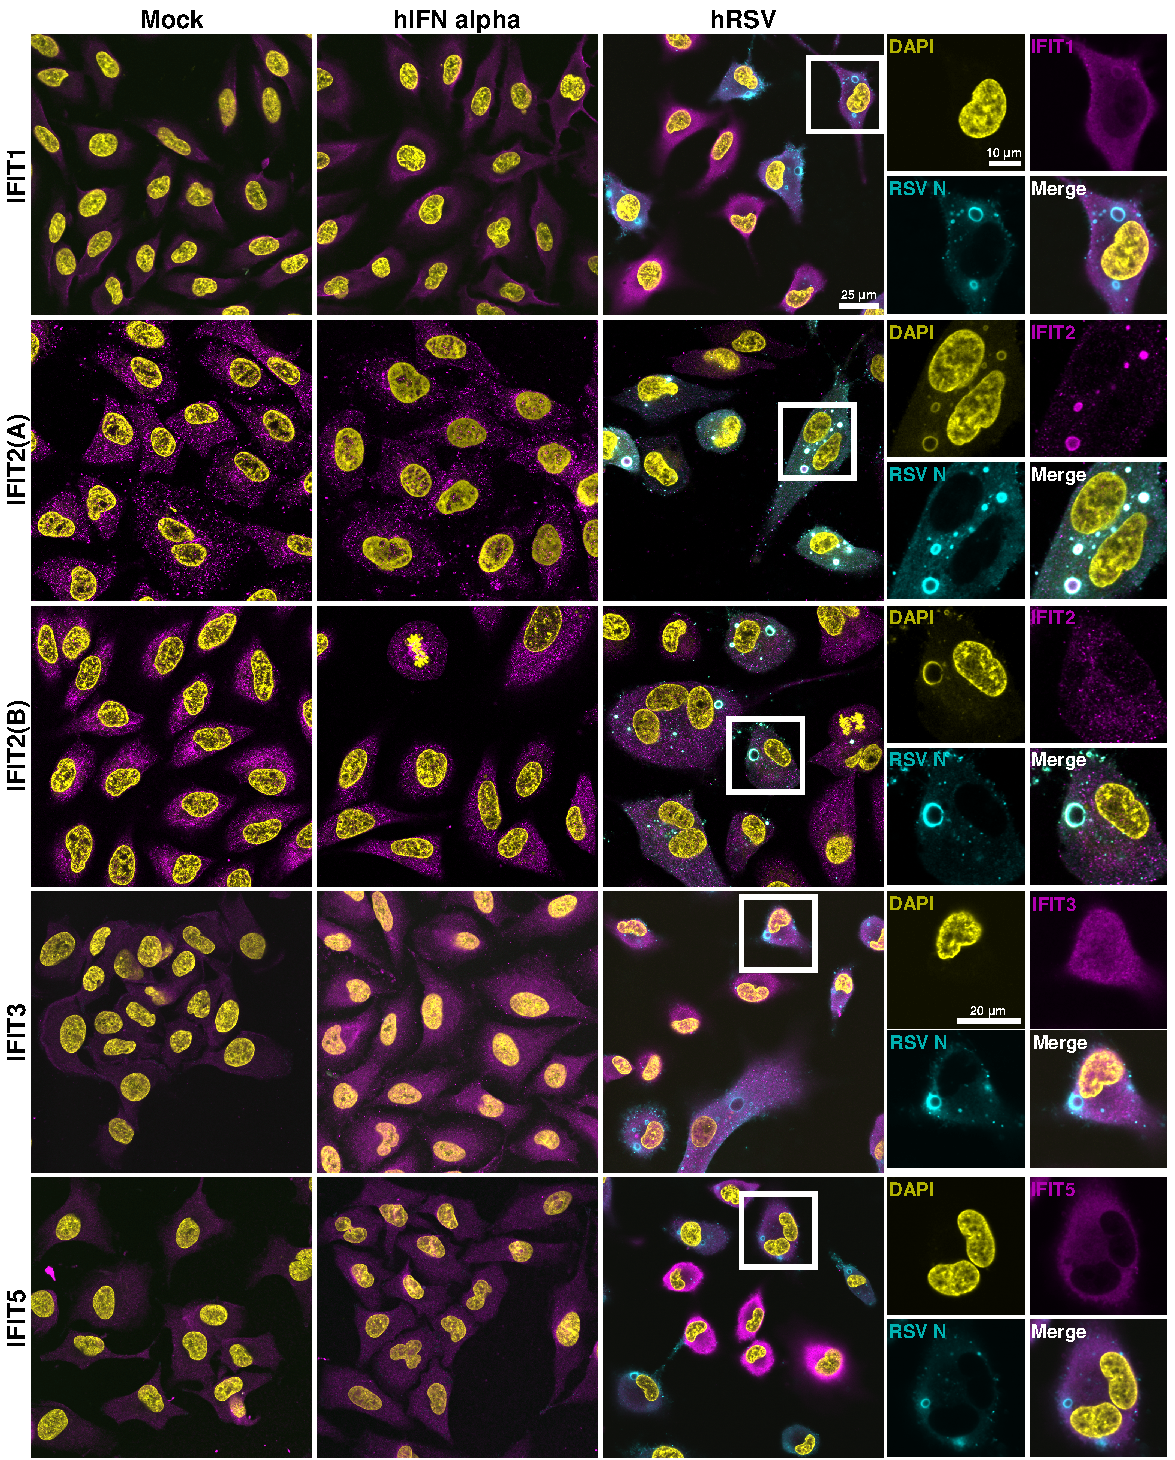
\includegraphics[width=1\linewidth]{08. Chapter 3/Figs/01. Localisation introduction/07. a549 merges.pdf}
    \caption[The Changes in Subcellular Localisation of Human IFITs in A549 Cells Subjected to hIFN\(\alpha\) or hRSV.]{\textbf{The Changes in Subcellular Localisation of Human IFITs in A549 Cells Subjected to hIFN\(\alpha\) or hRSV.} A549 cell were either mock treated, or treated with 1000 IU/mL of hIFN\(\alpha\) for 24 hours, or were infected with hRSV MOI 1 for 24 hours. Cells were fixed, and stained with DAPI (nuclei detection; yellow), anti-RSV N antibody (cyan), or with antibodies against IFIT proteins (magenta). Two antibodies against IFIT2 were used, termed IFIT2A and IFIT2B. Insets with magnified selections were created from infected images to more easily convey the underlying subcellular localisations.}
    \label{fig:The Changes in Subcellular Localisation of Human IFITs in A549 Cells Subjected to hIFNa or hRSV.}
\end{figure}


the results from bovine

\begin{figure}
    \centering
    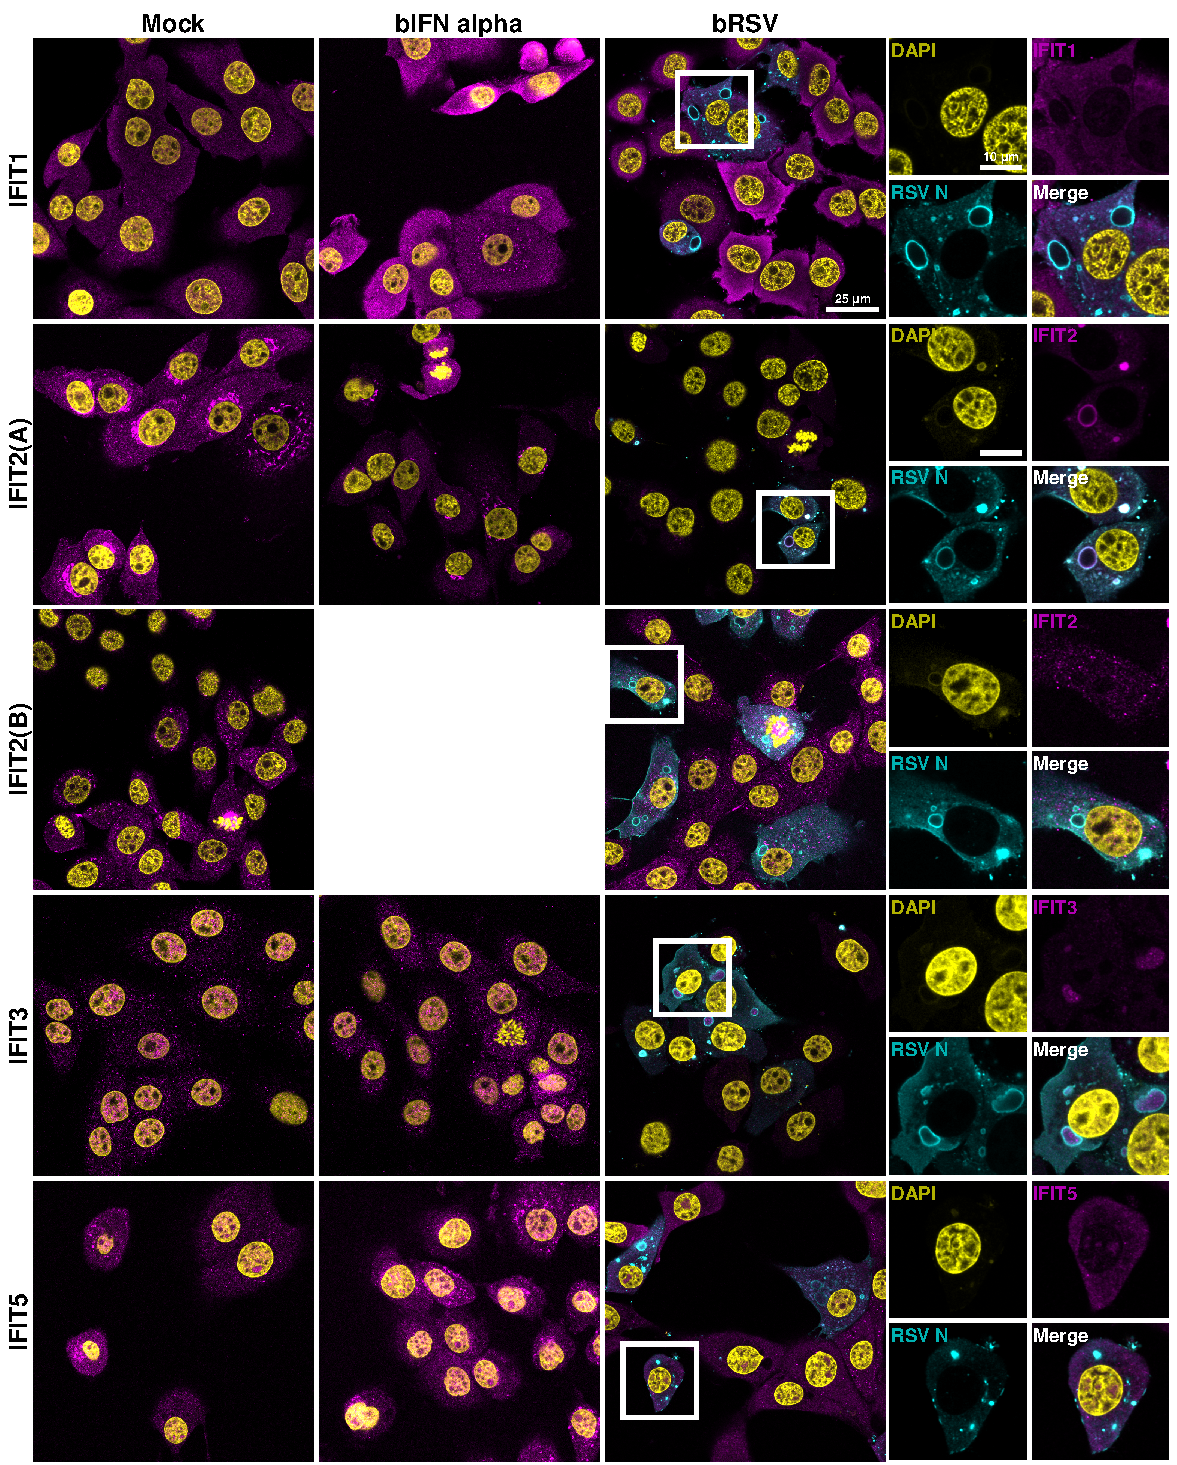
\includegraphics[width=1\linewidth]{08. Chapter 3/Figs/01. Localisation introduction/09. mdbk-merges-test.pdf}
    \caption[The Changes in Subcellular Localisation of Bovine IFITs in MDBK Cells Subjected to bIFN\(\alpha\) or bRSV.]{\textbf{The Changes in Subcellular Localisation of Bovine IFITs in MDBK Cells Subjected to bIFN\(\alpha\) or bRSV.} MDBK cell were either mock treated, or treated with 5 ng/mL of bIFN\(\alpha\) for 24 hours, or were infected with bRSV MOI 1 for 24 hours. Cells were fixed, and stained with DAPI (nuclei detection; yellow), anti-RSV N antibody (cyan), or with antibodies against IFIT proteins (magenta). Two antibodies against IFIT2 were used, termed IFIT2A and IFIT2B. Insets with magnified selections were created from infected images to more easily convey the underlying subcellular localisations.}
    \label{fig:The Changes in Subcellular Localisation of Bovine IFITs in MDBK Cells Subjected to bIFNa or bRSV}
\end{figure}

Seeing the potentially intersting results with IFIT colocalisation with RSV IBs, we systematically analysed 1727 IB sizes and their underlying interaction phenotype with the different IFIT proteins. We categorised the phenotypes solely based on the IFIT staining, but in the area of the image where a presence of inclusion body was confirmed by viral protein staining. Based on our observations, we decided to categorise the phenotypes in a following manner: \textbf{Diffusion} phenotype would be assigned if the IFIT signal would be equally spread through the area if interest; \textbf{Exclusion} phenotype, which would be assigned by a obvious, partial or full, decrease in signal within the boundry of IB; \textbf{Edge exclusion} phenotype would be assigned if the IFIT signal would be equally spread through the area if interest with the exeption of IB boundry, from which it would be excluded; \textbf{Inclusion} phenotype would be assignes if there was obvious increase in the IFIT signal within the boundry of IB; and \textbf{Colocalisation} phenotype, which would be assigned if the IFIT signal would be equally spread through the area if interest with the exeption of increased signal in the IB boundry. These main phenotypes were also simetimes supplemented by either their interaction, or the presence of spots within the IB boundry. For the former, a very common occurance was colocalisation accompanied by exclusion. This was when there was an obvious increase on the IB boundry compared to the surrounding signal, while also a marked decrease of signal from within the region of interest was present. For the latter, these spots were termed IBAGs, as we speculate that these structures could be inclusion body associated granules.

about setting gains menaing two images dont have the same intensities but signal is real. extending the useful range etc..  we cared about the observed phenotype. bilinear interpretation etc.

% introduction to ib stuff from my study
write about ib size statistics from my analysis

\begin{figure}
    \centering
    \includegraphics[width=1\linewidth]{08. Chapter 3/Figs/01. Localisation introduction/01. IB-zooms.pdf}
    \caption[Inclusion Bodies Within RSV Infected Cells: Zoom Sequence.]{\textbf{Inclusion Bodies Within RSV Infected Cells: Zoom Sequence.} A represerenative image of RSV infected cells detected using confocal microscopy. Cellular nuclei were stained with DAPI and are shown in yellow; RSV inclusion bodies are shown in cyan; and the cytoplasm is shown in magenta. Figure highlights a zoom sequence from a population of cells, into a single syncytia view, with lastly focusing at one individual inclusion body.}
    \label{fig:Inclusion Bodies Within RSV Infected Cells: Zoom Sequence}
\end{figure}

ibs are mainly spherical although expeptions happpen

\begin{figure}
    \begin{subfigure}{0.495\textwidth}
        \caption{}
        \includegraphics[width=\textwidth]{08. Chapter 3/Figs/01. Localisation introduction/02. heatmap_all.pdf} 
    \end{subfigure}
    \hfill
    \begin{subfigure}{0.495\textwidth}
        \caption{}
        \includegraphics[width=\textwidth]{08. Chapter 3/Figs/01. Localisation introduction/03. heatmap_a549.pdf}
    \end{subfigure}

    \medskip
    \begin{subfigure}{0.495\textwidth}
        \caption{}
        \includegraphics[width=\textwidth]{08. Chapter 3/Figs/01. Localisation introduction/04. heatmap_beas2b.pdf} 
    \end{subfigure}
    \hfill
    \begin{subfigure}{0.495\textwidth}
        \caption{}
        \includegraphics[width=\textwidth]{08. Chapter 3/Figs/01. Localisation introduction/05. heatmap_mdbk.pdf} 
    \end{subfigure}
    
    \caption[Size Characterization of Inclusion Bodies Across Different Cell Lines.]{\textbf{Size Characterization of Inclusion Bodies Across Different Cell Lines.} This figure presents the relationship between the measured area (\(\mu m^2\)) and diameter (\(\mu m\)) of individual inclusion bodies (IBs) as observed within the scope of this study. Additionally, the figure includes distinct population distributions depicted alongside the plots, representing (a) the aggregate of 1727 observations of IBs across all individual cell lines, (b) 1008 observations from the A549 cell line, (c) 99 observations from the BEAS2B cell line, and (d) 620 observations from the MDBK cell line. Contour plots are incorporated to elucidate the underlying density of individual IBs within the plots.}
    \label{fig:Size Characterization of Inclusion Bodies Across Different Cell Lines}  
\end{figure}

there is a clear difference in sizes detected in our study
compare to published and fj thesis
mdbk has more small ibs
each cell line seems to have also unusally large ibs


\begin{figure}
    \centering
    \includegraphics[width=1\linewidth]{08. Chapter 3/Figs/01. Localisation introduction/06. box-infection.pdf}
    \caption[boxplot of ib sizes per cell line.]{\textbf{boxplot of ib sizes per cell line.} this is the data from above but only area, to be able to compare it later}
    \label{fig:boxplot of ib sizes per cell line}
\end{figure}

5, 3, 2 areas